\documentclass{article}
\usepackage{amsmath}
\usepackage{graphicx}
\usepackage{float}
\usepackage{hyperref}
\usepackage{fancyvrb}
\usepackage{matlab-prettifier}
\setlength{\parindent}{0pt}

\title{CS663: Digital Image Processing - Homework 1}
\author{Harsh $\vert$ Pranav $\vert$ Swayam} 

\begin{document}

\maketitle
\section{Homework 1 - Question 6}

\subsection*{(a)}

The MATLAB code for this question is as follows:
\begin{lstlisting}[frame=single,numbers=left,style=Matlab-Pyglike,breaklines=true,postbreak=\mbox{\textcolor{red}{$\hookrightarrow$}\space}]    
n = 12;
choice = 1; %1 for ginput, else feed directly

if choice == 1
    for i = 1:n
        figure(1); imshow(im1/255); 
        [x1(i),y1(i)] = ginput(1);
        figure(2); imshow(im2/255); 
        [x2(i),y2(i)] = ginput(1);
    end
end

disp("Figure 1 goi1 selected points are:")
disp([x1, y1])
disp("Figure 2 goi2 selected points are:")
disp([x2, y2])
\end{lstlisting}

After running the above code, we get the following selected points for the two images:

\texttt{Terminal Out:\\
Figure 1 goi1 selected points are:\\
   202.3677  512.4066  277.6984  179.0214  316.9202  484.0798  264.9358  118.3210  424.9358  373.8852  367.3482  201.1226  256.7646  294.7412  251.4728  218.4767  219.4105  301.2782  175.8307  246.1809  178.3210   19.5661  210.0720  243.0681
}

\texttt{Figure 2 goi2 selected points are:\\
   236.6089  570.6167  313.8074  212.9514  353.0292  537.3093  299.1770  150.6946  467.2704  414.3521  406.2588  162.5233  277.9319  313.7296  271.0837  238.0875  238.7101  321.5117  192.6401  266.4144  191.3949   32.0175  230.3054  255.2082
}

\subsection*{(b)}

The MATLAB code for this question is as follows:
\begin{lstlisting}[frame=single,numbers=left,style=Matlab-Pyglike,breaklines=true,postbreak=\mbox{\textcolor{red}{$\hookrightarrow$}\space}]
P2 = [x2; y2; ones(1,n)];
P1 = [x1; y1; ones(1,n)];
A = P2*P1'*inv(P1*P1'); % Moore-Penrose pseudo-inverse

disp("Matrix A:")
disp(A);
\end{lstlisting}

After running the above code, we get the following matrix $A$:

\texttt{Terminal Out:\\
Matrix A:\\
\hspace*{2em}1.1047\hspace*{1.5em}-0.0012\hspace*{2.5em}1.2435\\
\hspace*{1.5em}-0.0032\hspace*{2em}1.0283\hspace*{2em}12.6563\\
\hspace*{2em}\hspace*{2.5em}0\hspace*{2em}\hspace*{2.5em}0\hspace*{2em}\hspace*{0.5em}1.0000}

Hence, the image \texttt{goi1} was transformed using the rotation, scaling, shearing and translation transformations to get the image \texttt{goi2}. This can be mathematically achieved using the matrix $A$.

\subsection*{(c)}

The MATLAB code for this question is as follows:
\begin{lstlisting}[frame=single,numbers=left,style=Matlab-Pyglike,breaklines=true,postbreak=\mbox{\textcolor{red}{$\hookrightarrow$}\space}]
im3 = zeros(size(im1));

for i = 1:H 
    for j = 1:W 
        dxy = A\[j i 1]'; 
        xx = round(dxy(1)); 
        yy = round(dxy(2)); 
        
        if xx > 0 && xx <= W && yy > 0 && yy <= H 
            im3(i,j) = im1(yy,xx); % nearest neighbor
        end
    end
end

figure(1); imshow(im1/255);
figure(2); imshow(im2/255);
figure(3); imshow(im3/255);

% Save all the images
saveas(figure(1), 'nn_im1.png');
saveas(figure(2), 'nn_im2.png');
saveas(figure(3), 'nn_im3.png');
\end{lstlisting}

The images obtained after the nearest neighbor interpolation are as follows:
\begin{figure}[htbp]
    \centering
    \begin{minipage}[b]{0.45\textwidth}
        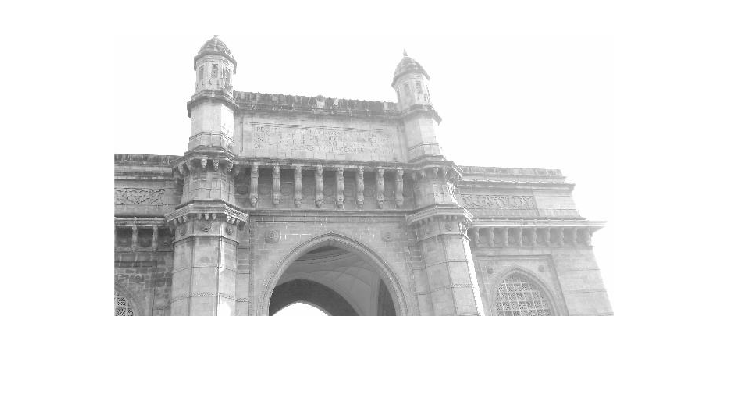
\includegraphics[width=\textwidth]{nn_im1.png}
        \caption{\texttt{goi1}}
    \end{minipage}
    % \hfill
    \begin{minipage}[b]{0.45\textwidth}
        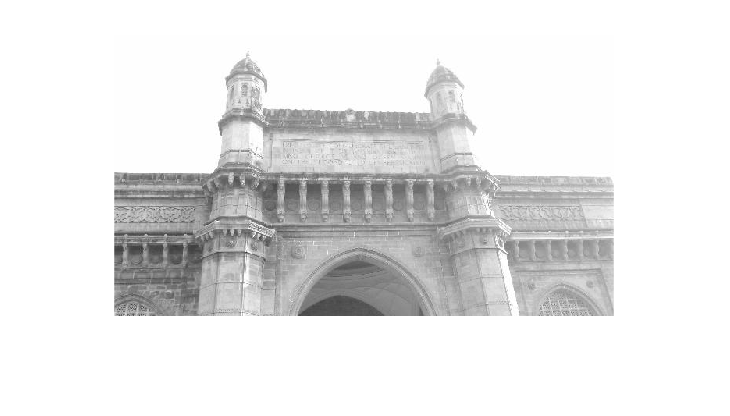
\includegraphics[width=\textwidth]{nn_im2.png}
        \caption{\texttt{goi2}}
    \end{minipage}
    % \hfill    
\end{figure}
\begin{figure}[!htb]
    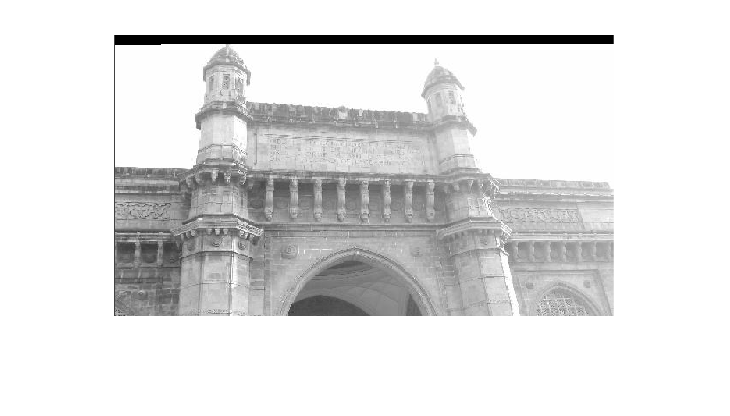
\includegraphics[width=\textwidth]{nn_im3.png}
    \caption{Interpolated Image (Nearest Neighbor)}
\end{figure}

\clearpage
\subsection*{(d)}

The MATLAB code for this question is as follows:
\begin{lstlisting}[frame=single,numbers=left,style=Matlab-Pyglike,breaklines=true,postbreak=\mbox{\textcolor{red}{$\hookrightarrow$}\space}]
im4 = zeros(size(im1));

for i = 1:H 
    for j = 1:W 
        dxy = A\[j i 1]'; 
        xx = round(dxy(1)); 
        yy = round(dxy(2)); 
        
        if xx > 0 && xx <= W && yy > 0 && yy <= H 
            w1 = (xx+1-dxy(1))*(yy+1-dxy(2)); % bilinear
            w4 = (dxy(1)-xx)*(dxy(2)-yy);
            w3 = (yy+1-dxy(2))*(dxy(1)-xx);
            w2 = (xx+1-dxy(1))*(dxy(2)-yy);
            im4(i,j) = im1(yy,xx)*w1+im1(yy+1,xx)*w2+im1(yy,xx+1)*w3+im1(yy+1,xx+1)*w4; 
        end
    end
end

figure(1); imshow(im1/255);
figure(2); imshow(im2/255);
figure(3); imshow(im4/255);

% Save all the images
saveas(figure(1), 'bilinear_im1.png');
saveas(figure(2), 'bilinear_im2.png');
saveas(figure(3), 'bilinear_im4.png');
\end{lstlisting}

The images obtained after the bilinear interpolation are as follows:
\begin{figure}[htbp]
    \centering
    \begin{minipage}[b]{0.45\textwidth}
        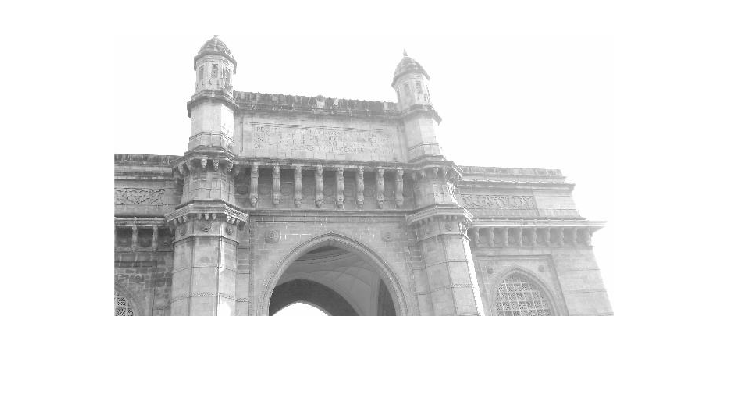
\includegraphics[width=\textwidth]{bilinear_im1.png}
        \caption{\texttt{goi1}}
    \end{minipage}
    % \hfill
    \begin{minipage}[b]{0.45\textwidth}
        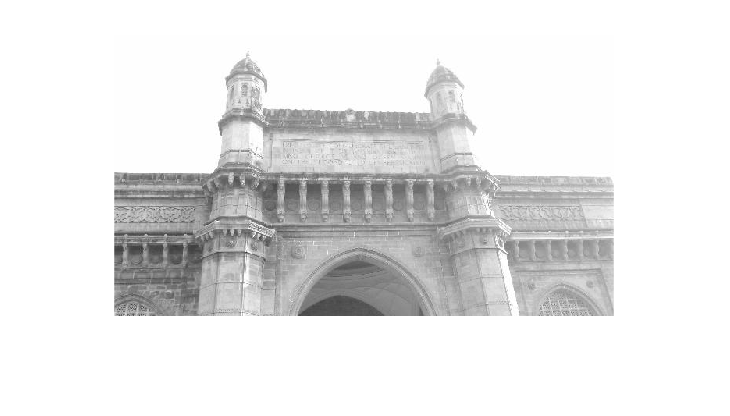
\includegraphics[width=\textwidth]{bilinear_im2.png}
        \caption{\texttt{goi2}}
    \end{minipage}
    % \hfill
\end{figure}
\begin{figure}[!htb]
    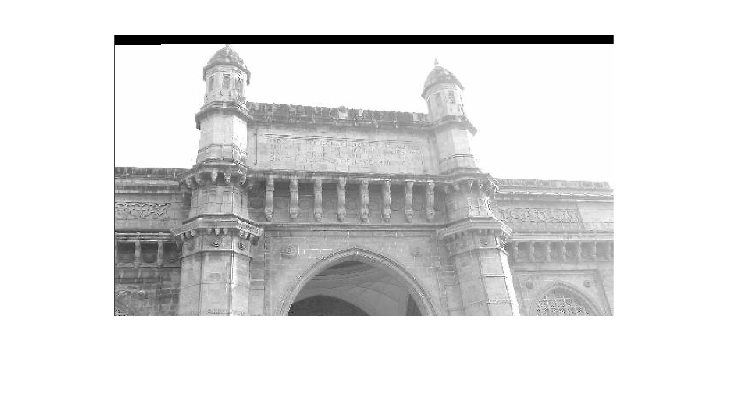
\includegraphics[width=\textwidth]{bilinear_im4.png}
    \caption{Interpolated Image (Bilinear)}
\end{figure}

\subsection*{(e)}
For estimating the affine transformation matrix, we need at least three non-collinear points. 

\vspace{5pt}
If all the selected points are collinear, then the following issues may arise:
\begin{enumerate}
\item The system of equations we formed to solve for the affine transformation matrix becomes \textit{underdetermined}, that there is not enough independent equations to uniquely solve for all parameters.
\item The computation will not capture any affine transformation that includes rotations, scaling, or translations.
\item The affine transformation cannot be estimated accurately because the equations would not span the required two-dimensional space. It essentially becomes a problem in one-dimensional space along the line.
\end{enumerate} 

\end{document}